\documentclass[a4paper,10pt]{article}
%\documentclass[a4paper,10pt]{scrartcl}

\usepackage[utf8]{inputenc}
\usepackage{enumerate}	
\usepackage{graphicx}
\usepackage{pdfpages}

\usepackage[acronym,toc]{glossaries} % nomain, if you define glossaries in a file, and you use \include{INP-00-glossary}
\documentclass[a4paper,10pt]{article}
\usepackage[utf8]{inputenc}
\usepackage{hyperref}
\usepackage[authoryear, round]{natbib}

% Title Page
\title{Glossary of Terms}
\author{}

\begin{document}
\maketitle

There are various glossaries related to MSE, stock assessment and risk.
 
\section{MSE}
  The main reference for terminology is in \href{http://icesjms.oxfordjournals.org/content/64/4/618.abstract}{\cite{rademeyer2007tips}}
  
\section{tRFMOs}

Some of the tRFMOs have their own glossaries
  %CCSBT \url{http://cran.r-project.org/web/packages/kobe}\\ 
  %IATTC \url{http://cran.r-project.org/web/packages/kobe}\\
  ICCAT \url{http://www.iccat.int/Documents/SCRS/Other/glossary.pdf}\\
  IOTC  \url{http://www.iotc.org/files/proceedings/2012/sc/IOTC-2012-SC15-INF03.pdf}\\
  %WCPFC \url{http://cran.r-project.org/web/packages/kobe}\\
  
\section{Risk}

  The International Organization for Standardization (ISO) is the world’s largest developer of voluntary International Standards. 
  International Standards give state of the art specifications for products, services and good practice, helping to 
  make industry more efficient and effective. Developed through global consensus, they help to break down barriers to international trade.
  They have a standard for Risk Management see

  ISO 31000:2009 \url{http://www.iso.org/iso/catalogue_detail?csnumber=43170}


\bibliographystyle{abbrvnat}
\bibliography{refs}

\end{document}          

\makeglossaries

\usepackage{hyperref}	

\usepackage{multibib}
\usepackage[authoryear, round]{natbib}

\newcites{peer}{Peer Review}
\newcites{scrs}{SCRS}
\newcites{peerInprep}{Peer Review}
\newcites{scrsInprep}{SCRS}
\newcites{software}{R Packages}


\title{GBYP MSE}

\begin{document}
\maketitle

This document summarises work being conducted in relation to the \gls{MSE} tasks identified at the  
\textbf{Meeting on Bluefin Stock Assessment Methods} (Gloucester, Massachusetts, United States July 20 to 22, 2013).

A variety of papers have been written or will be written on \gls{RA} and the MSE.  The objective of this document is to identify and propose collaborative 
papers (SCRS and \textbf{peer-reviewed}) to take this work forward and provide a bibliography.

MSE work being conducted for by the SCRS for other stocks summarised in a separate document.

All software and code will be open source and made available on the \href{http://rscloud.iccat.int}{ICCAT cloud server} to 
allow collaborative working both within the SCRC and between the scientific committees of other \glspl{RFMO}

\tableofcontents

\subsection{Risk Analysis}

A qualitative Risk Assessment has been conducted with members of the SCRS and the Commission under
Phases II and III; under Phases IV and subsequent phases the intention is to conduct quantitative analyses
to identify the main sources of uncertainty that should be developed as \glspl{OM} and 
then to review the process.

There are a variety of quantitative techniques that could be applied, from the relatively simple (e.g. elasticity and sensitivity analyses)
to complex approaches such as MSE. In the first instance it is intended to use a range of simple techniques to identify scenarios for use in the 
MSE. The approaches will then be reviewed in a peer review paper. 

Various papers peer review papers are being written and planed under the the GBYP, i.e.
papers i) reviewing historical sources of uncertainty considered \citepeer{fromentin2014spectre}
ii) Identification and prioritisation of uncertainties \citepeerInprep{leach2014elicit};
iii) Identification of the major sensitivities \citescrs{kell2014sense}; iv)  
simple methods based on life history relationships \citepeerInprep{kellInprepElas};
vii) a comparison of the relative importance of the values of information and control \citepeerInprep{gbypInprep1}; and 
iv) a review Paper summarising the lessons learnt \citepeerInprep{gbypInprep2}.

\subsection{MSE}

The Relative Value-of-Information for Model Based and Empirical Management Procedures:  A Mediterranean bluefin example 
\citescrs{bft2014afsmse}. 


\subsubsection{Operating Model}

Which Came First? The Chicken, The Egg or The Tortilla \citescrs{kell2014srr}.

Population and Stock Hypotheses for North Atlantic Bluefin Tuna \citescrs{kell2014pop}.
A Comparison of Model Based and Model Free Harvest Control Rules Using Management Strategy Evalution For North Atlantic Bluefin Tuna 
\citescrs{kell2014mp}.

 
\subsubsection{Management Proceedure}

A Comparison of Model Based and Model Free Harvest Control Rules Using Management Strategy Evalution For North Atlantic Bluefin Tuna
\citescrs{kell2014mp}

\newpage\clearpage
\section{Software}
\bibliographystylesoftware{abbrvnat}
\bibliographysoftware{refs}

\section{Papers in Preparation}
\bibliographystylescrsInprep{abbrvnat}
\bibliographyscrsInprep{refs}

\bibliographystylepeerInprep{abbrvnat}
\bibliographypeerInprep{refs}

\newpage\clearpage
\section{References}
\bibliographystylescrs{abbrvnat}
\bibliographyscrs{refs}

\bibliographystylepeer{abbrvnat}
\bibliographypeer{refs}


\section{Glossary}
\newpage\printglossaries


\newpage
\section{GBYP Modelling Tasks}
Identified at Gloucester, Massachusetts, United States – July 20 to 22, 2013



\subsection*{Outline: Detailed Work Plan for Conducting the Management Strategy Evaluation}
\label{sub:outline}

This section outlines, in tabular form, a schedule for the work required to conduct the 2014 and 2015 assessments and then 
to evaluate a management procedure using an operating model for Atlantic bluefin. A detailed work plan, based on this schedule, 
will be developed for presentation at the SCRS plenary. Following endorsement by the SCRS, a budget will be proposed for 
presentation to the Commission. To implement the operating model, it is essential that contracts for providing external 
support for a number of years are awarded. It is also essential to establish a core steering group to oversee the work.

\subsubsection*{2013}

\begin{enumerate}
\item Discussion of alternative mixing structures in broad terms SCRS paper with key contributors
\item Clarification of standard inputs to standard separate west/east assessments.
Use ICCAT meeting to facilitate with those most familiar with data (Terms of Reference document)
Table of information available
\item Clarification on data availability for mixing and stock structure related data for more complex stock assessments.
Genetic, microconstituents, tags (archival, conventional, other)
\item Identification of major sensitivities for both separate and mixed stock assessments (e.g., M, fecundity schedule, SRR and alternative mechanism of population regulation)
\item Use Risk assessment paper on qualitative identification of uncertainty (written under GBYP modelling contract) to inform OM scenarios, i.e., SCRS paper with key contributors.
\item Identification of those who will be taking both assessment approaches further forward
Consistent, core group over a multi-year timeline
\item Support capacity development for conduct, understanding and use of MSE in adoption of Harvest Control Rules for the Atlantic bluefin fisheries through:
ICES/ICCAT MSE training in (Dec. 2013) to facilitate capacity building for CPC scientific delegations; 
Take advantage of GEF/FAO Areas Beyond National Jurisdiction Tuna Program funds intended to accelerate the joint tuna RFMO working group for MSE development and management /stakeholder / science (jargon-free) dialogue.
Conduct a ‘side event’(SCRS Chairman to co-ordinate) at the 2013 Commission meeting open to CPCs and stakeholder groups, drawing upon the experience at CCSBT to initiate the management / science/ stakeholder dialogue. 
\end{enumerate}


\subsubsection*{2014} 

For bluefin session
\begin{enumerate}
\item Eastern assessment update 
Post-bluefin; ideally follows bluefin session
\item Review of updated separate assessment approaches
\item Review of initial mixed stock models and refinement of alternative mixing structure scenarios
\item Tool for visualizing movement
\item Meeting including stakeholders (finalise at 2013 Commission meeting)
\end{enumerate}

\subsubsection*{2015}


For bluefin session
\begin{enumerate}
\item Data guillotine – finalisation of data to be considered for operating model development for MP testing (back reference); includes data update for assessments for that year.
\item Updated catch limit advice for both East and West based on revised separate assessments, and possibly also mixed stock models
\end{enumerate}

\subsubsection*{2016}

For separate meeting (Jan-Feb 2016)
\begin{enumerate}
\item Agreement on operating model specifications (conditioning)
\item Agreement on data for use in MPs
Subset of OM data
\item Initial agreement on objectives and performance statistics (other stakeholders need to be included in these discussions)
\item Specifications and schedule for coding
Early in year
\item Circulation of code to allow alternative MP developers to plug-in and test their candidate MPs
Bluefin session
\item Refinement of MP testing procedures
\item Interaction with stakeholders for feedback based on initial results from developers
\end{enumerate}

\subsubsection*{2017}

Bluefin session
\begin{enumerate}
\item Review of further results from developers
\item Development of final recommendations to Commission on MP to adopt, together with its associated data inputs.
\end{enumerate}



\newpage
\section{Data Preparatory Meeting} 
(Madrid, Spain - May 5 to 10, 2014)

%Tasks under GBYP Modelling for 2013, identified at Gloucester Meeting


\subsection{Objectives}

In 2013 the SCRS elaborated a work plan for 2014 which included a data preparatory meeting to incorporate the new catch and effort information in ICCAT databases and continuing working on new modeling platforms and inputs in a view to minimize uncertainties in the 2015 and ongoing assessments. The work plan approved by the SCRS did not include an update of the stock assessment in 2014, as stated by the ICCAT Recommendation [12-03] for the eastern Atlantic and Mediterranean bluefin tuna. This decision was based in the lack of SCRS resources for conducting the update and undertaking the difficult task of preparing the 2015 assessment. 

Nevertheless, the Commission at its 23th Regular Meeting requested the SCRS to implement Rec. [12-03], i.e., to update the stock assessment of East Atlantic and Mediterannean bluefin tuna. The following year the Commission also adopted Recommendation 13-09 which states: “In 2014, the SCRS will update the stock assessment for bluefin tuna for the western Atlantic stock”.

Hence, the work plan developed by the Bluefin tuna species group for 2014 has needed to be modified to include in 2014 an update of both the West and the East Atlantic and Mediterranean stock assessments and the corresponding data preparatory work. The new work plan elaborated by the Bluefin rapporteurs and the SCRS Chair is attached as Annex 1. 

Following the revised work plan the objectives of this data preparatory meeting are the following: 

\begin{enumerate}[1.]
\item Update fishery indicators in accordance Rec. [12-03], paragraph. 50. 
\item Revise Task II by validating and integrating the catch at size statistics with new information from farms and other sources of information. 
\item Update the length-weight relationship for both stocks, i.e. Western and Eastern / Mediterranean stocks. 
\item Define the procedure to prepare CAS, CAA, WAA (total and per fleet) using the new length-weight relationship. 
\item Review tagging past and recent data for bluefin tuna.
\item Complete outstanding tasks from the Biological Parameters meeting in Tenerife (age-length relationships, morphometric conversions, natural mortality, reproduction, etc.). 
\end{enumerate}

\subsection{Tentative Agenda}

\begin{enumerate}[1.]
\item Opening, adoption of the Agenda and meeting arrangements.
\item Review of historical and new information on biology
\item Review of old and new Task I after the incorporation of new information from GBYP and other sources
\item Review of old and new Task II catch/effort data after the incorporation of new information from GBYP and other sources 
\item Review of old and new Task II size data 

\begin{enumerate}[5.1]
\item 5.1 Review of new information from farms and other sources
\item 5.2 Validation of the procedure followed to incorporate the information from farms and other sources into the ICCAT data base
\end{enumerate}

\item Definition of a new procedure to estimate CAS, CAA and WAA using new information validated by the Group
\item Review of available indices of relative abundance by fleet 
\item Definition of data inputs and specifications for the 2014 update assessment and advice framework.  
\item Identification of the evaluation team and definition of the revision procedure
\item  Develop a web app from the R-VPA2-BOX interface
\item Responses to the Commission
\begin{enumerate}[11.1]
\item Develop updated growth tables
\end{enumerate}
\item Recommendations
\item Other matters
\item Adoption of the report and closure
\end{enumerate}

\subsection{2014 Bluefin Tuna Work Plan}

Recommendation [10-04] states “In 2012, and thereafter every three years, the SCRS will conduct a stock assessment for bluefin tuna for the western Atlantic and eastern Atlantic and Mediterranean and provide advice to the Commission on the appropriate management measures, inter alia, on total allowable catch levels for those stocks for future years.” 

The Atlantic-wide Research Program for Bluefin tuna (GBYP) and various National programs have produced, and continue to produce, a great deal of new information on the biology and fisheries for bluefin tuna. In preparation for the planned 2015 assessment, time and resources of the SCRS are thus required to validate these data and to incorporate them in the ICCAT database as well as working on updated biological parameters and new modeling approaches. Therefore, the SCRS planned for several meetings in the 2012 work plan. The first two took place in 2013 and aimed at updating the biological parameters and comparing various modeling platforms. For 2014, the SCRS planned a data preparatory meeting (5-10 May) to incorporate the new catch and effort information in ICCAT databases and continuing working on new modeling platforms. 

Recommendation [12-03] for the eastern Atlantic and Mediterranean bluefin tuna further states “In 2014 the SCRS will conduct an update of the stock assessment and provide advice to the Commission.../... Furthermore, the SCRS shall work towards the development of new assessment modeling approaches and inputs, in a view to minimize uncertainties, which shall be used in a stock assessment in 2015 and thereafter every three years.” Finally, at its last session the Commission also adopted Recommendation 13-09 which states: “In 2014, the SCRS will update the stock assessment for bluefin tuna for the western Atlantic stock”.

To accommodate priorities to improve the scientific advice by 2015 and the latest commission requests, the SCRS proposes the following workplan for 2014, adapted from the plan approved by the SCRS in 2013:

\begin{enumerate}[1.]
\item Conduct an Inter-sessional Preparatory Workshop in early 2014 (6 days) that will focus on the following: 
\begin{enumerate}[a)]
\item Update fishery indicators in accordance Rec. [12-03], paragraph. 50, except for the Spanish bait boat CPUE as their quota has been transferred to Spanish purse seiners since 2012. The Japanese CPUE will have to be split into two periods, before and after TAC implementation due to changes in spatial coverage of the fishery. 
\item Revise Task II by validating and integrating the catch at size statistics with new information from farms and other sources of information. 
\item Update the length-weight relationship for both stocks, i.e. Western and Eastern / Mediterranean stocks. 
\item Prepare CAS, CAA, WAA (total and per fleet) using the new length-weight relationship. 
\item Review tagging past and recent data for bluefin tuna.
\item Complete outstanding tasks from the Biological Parameters meeting in Tenerife (age-length relationships, morphometric conversions, natural mortality, reproduction, etc.). 
\end{enumerate}
\item Continue a series of workshops and related activities (to be sponsored by the GBYP and various national programs) in accordance with recommendations from the Biological Parameters Meeting (Tenerife) and the Bluefin Methods meeting (Gloucester) including:
\begin{enumerate}[a)]
\item Establish a reference collection for otoliths and hard parts and calibrate age estimates among readers.
\item Larval biology workshop.
\item Continue the development of new modeling platforms that can better take into account various sources of uncertainties.
\end{enumerate}
\item Update the 2012 assessments of western and eastern/Mediterranean bluefin tuna using, insofar as is possible, the methods used during 2012.
\end{enumerate}


There is thus a considerable amount of work to be done in 2014, i.e., validating and incorporating 10,000s of new files into the current ICCAT databases, calibrating and updating all the size and age conversion methods, updating previous assessments and continuing the development of new modeling platforms.

The work plan for 2014 is detailed in a table of the main tasks, responsibilities, deadlines and priorities which is provided as an annex to this document. The first priority will be to conduct an update of the 2012 stock assessment for western and eastern/Mediterranean stocks using catch data and abundance indices updated through 2013. The second priority will be to incorporate the new information (trade, farms, biology) into the Task I and Task II data base (catch, catch-at-size, catch-at-age, weight-at-age). A preliminary assessment of the eastern/Mediterranean stock based on these revised Task I and Task 2 data will be attempted, but priority will be given to completing the update assessment stipulated by the relevant Commission Recommendations”. This line of priorities defines the order of the work that will be undertaken. Each priority must be completed in order for the group to move forward to the next step. The SCRS proposes that an additional inter-sessional meeting be planned in September 2014, during the species group meetings, to conduct the update of the 2012 stock assessment of eastern and western Atlantic stocks and, if time permits, a preliminary new assessment for the eastern stock. . This new preliminary stock assessment for the East will apply the current VPA software (VPA-2BOX) to the revised catch data using the new information (farm, trade, biological parameters). Initial ‘pilot’ updates of the 2012 SA (east and west) and the new preliminary SA for the East will be completed before the species group by the co-chairs and volunteer scientists and circulated prior to the species group meeting in September as an SCRS document. Any proposed revisions to the assessment will be addressed during the beginning of the Bluefin species group meeting to allow time for any additional runs and incorporation of the results into the executive summary. However, even if the new data are available this new stock assessment is unlikely to reduce substantially most of the unquantified uncertainties.

The following table summarized the activities defined in the work plan and its priorities. 


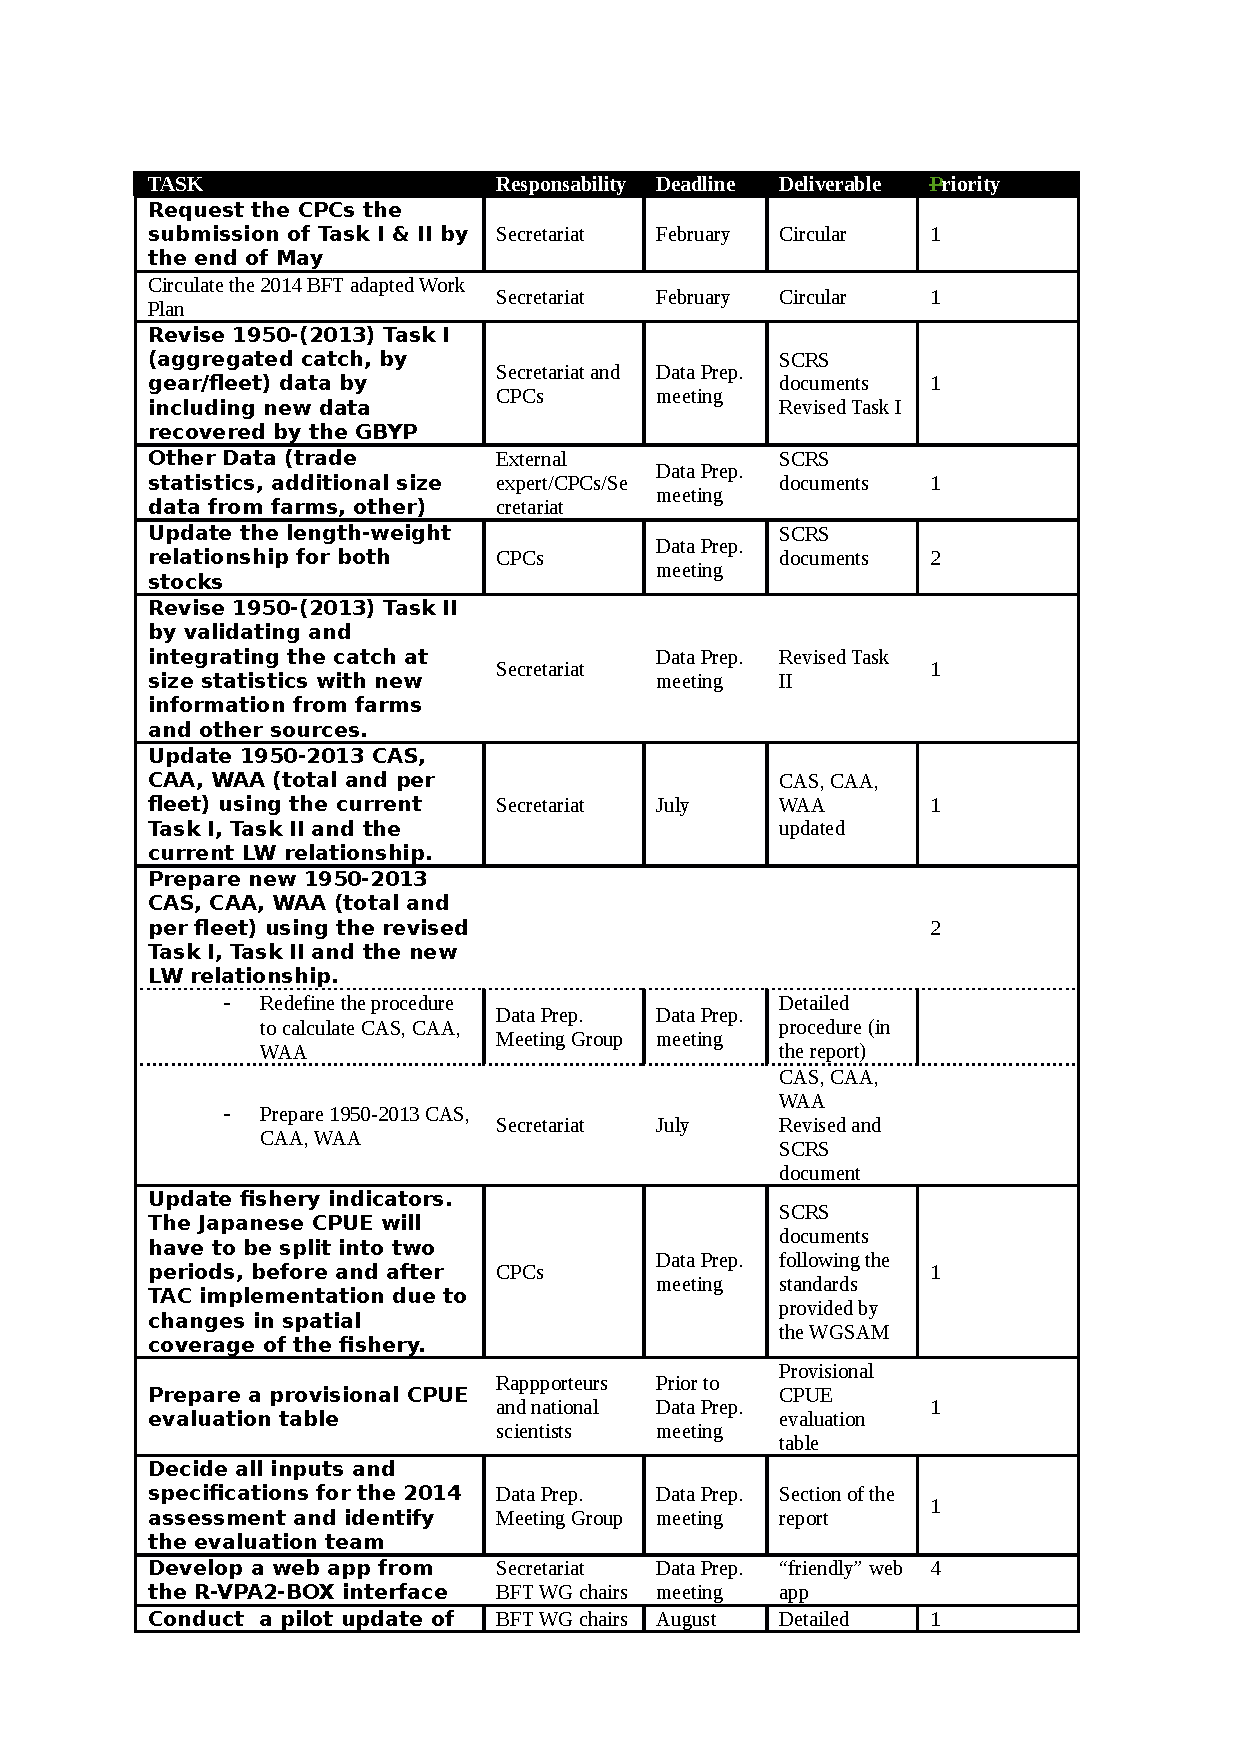
\includepdf[pages={1,2},lastpage=2]{dataPrepTab.pdf}


\end{document}


\clearpage\newpage
\section{Work in Progress}

A variety of tasks were proposed at GBYP Modelling for by year to take the work forward.

\begin{enumerate}[2013]
 \item 
\begin{enumerate}
\item Discussion of alternative mixing structures in broad terms SCRS paper with key contributors. 
%\textbf{[SCRS paper 1]}
\item Clarification of standard inputs to standard separate west/east assessments. Use ICCAT meeting to facilitate with those most familiar with data (Terms of Reference document). Table of information available 
%\textbf{[?]}
\item Clarification on data availability for mixing and stock structure related data for more complex stock assessments. Genetic, microconstituents, tags (archival, conventional, other) 
%\textbf{[SCRS paper 1]}
\item Identification of major sensitivities for both separate and mixed stock assessments (e.g., M, fecundity schedule, SRR and alternative mechanism of population regulation) 
%\textbf{[SCRS paper 1, Peer Review Paper 1, Peer Review Paper 2]}
\item Use Risk assessment paper on qualitative identification of uncertainty (written under GBYP modelling contract) to inform OM scenarios, i.e., SCRS paper with key contributors. 
%\textbf{[Peer Review Paper 1, GBYP Contract I]}
\item Identification of those who will be taking both assessment approaches further forward Consistent, core group over a multi-year timeline 
%\textbf{[?]}
\item Support capacity development for conduct, understanding and use of MSE in adoption of Harvest Control Rules for the Atlantic bluefin fisheries through:
\begin{enumerate}
\item ICES/ICCAT MSE training in (Dec. 2013) to facilitate capacity building for CPC scientific delegations; 
%\textbf{[ICES/ICCAT Training Course]}
\item Take advantage of GEF/FAO Areas Beyond National Jurisdiction Tuna Program funds intended to accelerate the joint tuna RFMO working group for MSE development and management /stakeholder / science (jargon-free) dialogue. 
%\textbf{[wait and see]}
\item Conduct a ‘side event’(SCRS Chairman to co-ordinate) at the 2013 Commission meeting open to CPCs and stakeholder groups, drawing upon the experience at CCSBT to initiate the management / science/ stakeholder dialogue. 
%\textbf{[!]}
\end{enumerate}
\end{enumerate}

\item

For bluefin session
\begin{enumerate}
\item Eastern assessment update 
Post-bluefin; ideally follows bluefin session
\item Review of updated separate assessment approaches
\item Review of initial mixed stock models and refinement of alternative mixing structure scenarios
\item Tool for visualizing movement
\item Meeting including stakeholders (finalise at 2013 Commission meeting)
\end{enumerate}
\end{enumerate}

